\subsection{Zadania}

Zakładamy, że wszystkie rozpatrywane przestrzenie topologiczne są drogowo spójne.

\begin{problem}
  Uzasadnij, że składanie dróg spełnia następujący warunek skreśleń: jeśli $f_0g_0\sim f_1g_1$ oraz $g_0\sim g_1$, to $f_0\sim f_1$.
\end{problem}

\begin{solution}
  Niech $g_0$ będzie drogą o początku w $x_0$. Zauważmy, że podobnie jak w pętlach
  $$f_0\sim f_0 x_0\sim f_0(g_0g_0^{-1})\sim (f_0g_0)g_0^{-1}.$$
  Wiemy, że $(f_0g_0)\sim f_1g_1$. Z drugiej strony, skoro $g_0\sim g_1$, to idąc "od tyłu" po homotopii między tymi drogami, tzn. $G'(s, t)=G(1-s, t)$, dostajemy homotopię między $g_0^{-1}$ a $g_1^{-1}$. Czyli
  $$f_0\sim f_0x_0\sim (f_0g_0)g_0^{-1}\sim (f_1g_1)g_1^{-1}\sim f_1(g_1g_1^{-1})\sim f_1x_0\sim f_1$$
\end{solution}

\begin{problem}
  Pokaż bezpośrednio z definicji, że dla pętli $f,g$ w $X$ zbazowanych w $x_0\in X$ zachodzi równoważność $f\sim g\iff f g^{-1}\sim x_0$, gdzie $x_0$ to pętla stała zbazowana w $x_0$, zaś $g^{-1}$ to pętla odwrotna do $g$.
\end{problem}

\begin{solution}
  $\implies$
  
  Zaczynamy od napisania homotopii 
  $$fg^{-1} \sim gg^{-1},$$ 
  czyli funkcji
  $$G(s, t)=H(s, 1-t)g(1-s).$$ 
  Potem, korzystając ze wzoru w dowodzie twierdzenia \ref{twierdzenie:1.4} dostajemy homotopię $gg^{-1}\sim x_0$. To daje nam 
  $$fg^{-1}\sim gg^{-1}\sim x_0$$ 
  tak jak chcieliśmy.

  $\impliedby$

  Niech $H(s, t)$ będzie homotopią między $fg^{-1}$ a $x_0$. Wtedy $H(s, t)g(s)$ będzie homotopią między $fg^{-1}g$ a $x_0g$, co po skorzystaniu ze wzoru użytego w twierdzeniu \ref{twierdzenie:1.4} daje
  $$f\sim fg^{-1}g\sim x_0g.$$
  Pozostaje napisać homotopię $x_0g\sim g$. Będzie to funkcja stale równa $x_0$ na odcinku $[0, (1-t)/2]$ oraz $g(s)$ na pozostałej długości przedziału $[0,1]$. Wzorem, wygląda to następująco:
  $$G(s, t)=\begin{cases}
  x_0&s\leq \frac{1-t}{2}\\ g\left(\left(s-\frac{1-t}{2}\right)\frac{2}{1+t}\right)&\frac{1-t}{2}<s\end{cases}$$
\end{solution}

\begin{problem}
  Uzasadnij, że dla dowolnej przestrzeni topologicznej $X$ następujące trzy warunki są równoważne:
  \begin{enumerate}[label=\alph*)]
    \item każde odwzorowanie $S^1\to X$ jest homotopijne ze stałym
    \item każde odwzorowanie $S^1\to X$ rozszerza się do odwzorowania $D^2\to X$, gdzie $D^2$ to $2$-wymiarowy dysk, którego brzegiem jest nasze $S^1$
    \item $\pi_1(X, x_0)=0$ dla dowolnego $x_0\in X$
  \end{enumerate}
  Wywnioskuj stąd, że przestrzeń $X$ jest jednospójna wtedy i tylko wtedy gdy wszystkie odwzorowania $S^1\to X$ są homotopijne.
\end{problem}

\begin{solution}
  $a)\implies b)$

  Utożsamimy $S^1$ z okręgiem jednostkowym na płaszczyźnie, czyli zbiorem punktów 
  $$\{(\cos\theta, \sin\theta)\;:\;\theta\in[0,2\pi)\}.$$
  Wtedy $D^2$ to zbiór
  $$\{(r\cos\theta, r\sin\theta)\;:\;\theta\in[0,2\pi), 0\leq r\leq 1\}=S^1\times [0,1]/ S^1\times\{0\}.$$
  Niech teraz $H(t, s)$ będzie homotopią między $f$ a odwzorowaniem stałym $c$. Wtedy
  $$F:D^2=S^1\times[0,1]/S^1\times\{0\}\to X$$
  jest zdefiniowane jako 
  $$F(s, t)=H(s, t)=f_t(s)$$

  $b)\implies a)$

  Weźmy dowolne odwzorowanie $f:S^1\to X$. Z $b)$ wiemy, że możemy je "zakleić". Niech $F:S^1\times [0,1]/S^1\times\{0\}=D^2\to X$ będzie rozszerzeniem $f$, dla którego $F(0,1)=x_1$, $F(x, 1)=f(x)$ oraz $F(x, 0)=c$ jest stałe niezależnie od wyboru $x$. 

  Napiszmy odwzorowanie 
  $$H(s, t)=F(s, 1-t),$$
  które jest homotopią między $f$ a "środkiem" dysku $c$. Jest to więc homotopia między odwzorowaniem $f$ a funkcją stale równą $c$.
  %Wystarczy tylko dodać tutaj odwzorowanie, które w sposób ciągły $F(0, 0)=c$ przesuwa na $F(0, 1)=x_0$. 

  $c)\implies a)$

  Dowolna pętlę możemy zinterpretować jako odwzorowanie $f:S^1\to X$. Niech $x_0=f(0)$. Z $c)$ wiemy, że $\pi_1(X, x_0)=0$, czyli $[x_0]=[f]$ i $f$ jest homotopijne z odwzorowaniem stale równym $x_0$.

  $a)\implies c)$

  Wybierzmy dowolne $x_0\in X$. Niech $f:S^1\to X$ będzie dowolnym odwzorowaniem takim, że $f(0)=f(1)=x_0$. Wiemy, że jest ono homotopijne z odwzorowaniem stałym $f\sim c$. Wystarczy teraz zauważyć, że homotopia między $f$ a $c$ daje również homotopię między $c$ a $x_0$. Czyli dowolna pętla $f:S^1\to X$ zbazowana w $x_0$ jest homotopijna z $x_0$. Stąd $\pi_1(X, x_0)=0$ dla dowolnego $x_0$.

  \begin{center}
    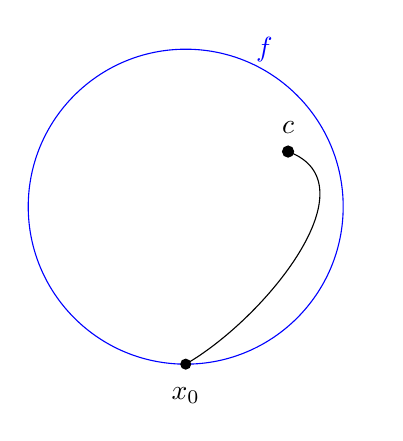
\begin{tikzpicture}
      \draw[blue] (0,0) circle (2);
      \fill (0, -2) circle (2pt);
      \draw (1.3, 0.7) circle (2pt);
      \draw (0,-2) to [out=30, in=-20] (1.3, 0.7);
      \fill (1.3, 0.7) circle (2pt);
      \node at (1.3, 1) {$c$};
      \node at (0,-2.4) {$x_0$};
      \node at (1, 2) {$\color{blue}f$};
    \end{tikzpicture}
  \end{center}

  Przestrzeń $X$ jest jednospójna, gdy jest drogowo spójna i ma trywialną grupę podstawową. Jednospójność w oczywisty sposób implikuje warunek $c)$ wyżej, z którego dostajemy, że dowolne dwa odwzorowania $S^1\to X$ są homotopijne z punktami stałymi, które możemy połączyć ($X$ łukowo spójne). 

  Z drugiej strony, jeśli dowolne dwa odwzorowania $S^1\to X$ są homotopijne, to w szczególności każde takie odwzorowanie jest homotopijne z odwzorowaniem stałym $x_0$ dla dowolnego $x_0\in X$. To daje łukową spójność $X$ oraz trywialność grupy podstawowej.
\end{solution}

\begin{problem}
  Jeśli $\pi_1X=0$, to każde dwie drogi łączące dowolnie wybrane dwa punkty $x_0, x_1\in X$ są homotopijne.
\end{problem}

\begin{solution}
  Niech $f, g$ będą drogami między $x_0$ a $x_1$. Wtedy $fg^{-1}$ będzie pętlą zbazowaną w $x_0$. Ponieważ $\pi_1X=0$, to $fg^{-1}\sim x_0$. Z zadania 2 wiemy, że wtedy $f\sim g$.
\end{solution}

\begin{problem}
  Mówimy, że przestrzeń topologiczna $X$ jest ściągalna, jeśli istnieje odwzorowanie $F:X\times I\to X$ takie, że $F(x, 0)=x$ oraz $F(x, 1)=x_0$ dla dowolnego $x$ oraz pewnego ustalonego $x_0$. Uzasadnij, że jeśli $X$ jest przestrzenią ściągalną, to jest też drogowo spójna, oraz $\pi_1X=0$ (innymi słowy, $X$ jest wtedy jednospójna).
\end{problem}

\begin{solution}
  Niech $x_1,x_2\in X$ będą dowolnymi punktami. Wówczas droga $f(t)=F(x_1, t)$ idzie z $x_1$ do $x_0$, a droga $g(t)=F(x_2, 1-t)$ idzie od $x_0$ do $x_2$. Łącząc obie te drogi dostajemy ścieżkę $x_1$ do $x_2$, czyli przestrzeń jest łukowo spójna.

  Weźmy teraz dowolną pętlę $f$ zbazowaną w punkcie $x_0$. Rozważmy homotopię $H(s, t)=F(f(s), t)$, która dla $t=0$ wynosi $f(s)$, a dla $t=1$ jest stale równa $x_0$. Z tego wynika, że $f\sim x_0$, czyli każda pętla jest homotopijna z elementem neutralnym $\pi_1X$ i grupa ta jest trywialna.
\end{solution}

\begin{problem}
  Uzasadnij, że każdy wypukły podzbiór w $\R^n$ jest ściągalny.
\end{problem}

\begin{solution}
  Wybierzmy dowolny punkt $x_0$ i z definicji zbioru wypukłego odcinek łączący $x_0$ z dowolnym innym punktem tego zbioru musi być zawarty w całości w tym zbiorze. Wystarczy napisać funkcję, która w sposób ciągły będzie przesuwać punkty po odcinkach łączących je z $x_0$.
\end{solution}

\begin{problem}
  Niech $T$ będzie skończonym \emph{drzewem}, tzn. spójnym skończonym grafem niezawierającym zamkniętych cykli krawędzi. Uzasadnij, że $\pi_1T=0$.
\end{problem}

\begin{solution}
  Jedyne pętle jakie znajdziemy w $T$ to pętla stała oraz pętle, które idą po wierzchołkach w jedną stronę i wracają po swoich śladach do punktu zaczepienia. Ten drugi rodzaj pętli to $ff^{-1}$ i jest homotopijne równy drodze stałej.
\end{solution}

\begin{problem}
  Uzasadnij, że homomorfizm $\phi_c:\pi_1(X, x_0)\to \pi_1(X, x_1)$ (związany ze zmianą punktu bazowego) zależy tylko od klasy homotopii drogi $d$ od $x_0$ do $x_1$.
\end{problem}
